\documentclass{beamer}
\usetheme{Warsaw}
\usepackage{hrslides}
\usepackage{graphicx}
\usepackage[space]{grffile}
\usepackage{listings}
\lstset{language=C,
basicstyle=\ttfamily\footnotesize,
frame=shadowbox,
mathescape=true,
showstringspaces=false,
showspaces=false,
breaklines=true}
\usepackage[utf8]{inputenc}

\title{Notions of computability}

\author{Dr. Giuseppe Maggiore}

\institute{Hogeschool Rotterdam \\ 
Rotterdam, Netherlands}

\date{}

\begin{document}
\maketitle

\SlideSection{Introduction}
\SlideSubSection{Lecture topics}
\begin{slide}{
\item Are there limits to what we can compute?
\item Are there limits to logical knowledge?
\item Are these two related?
}\end{slide}

\SlideSubSection{Gödel numbering}
\begin{slide}{
\item To work out the proofs of today we will build self-referential objects
\item We need to concisely represent programs, statements, etc.
\item We encode such objects as natural numbers
}\end{slide}

\begin{slide}{
\item This means that any statement within our system is now a natural number
\item ``Properties of statements'' $\Leftrightarrow$ ``properties of numbers''
\item There are many ways to define this encoding; we see Gödel's original
}\end{slide}

\begin{slide}{
\item First assign a unique natural number to each basic symbol in the language
\begin{itemize}
\item \texttt{if} $=0$
\item \texttt{var} $=1$
\item \texttt{,} $=2$
\item ...
\end{itemize}
}\end{slide}

\begin{slide}{
\item Given any formula $x_1,x_2,\dots,x_n$, $x_i$ is a number from the list above
\item $enc(x_1,\dots,x_n)=2^{x_1} \cdot3^{x_2} \cdot \dots \cdot p_n^{x_n}$
\item $p_n$ is the $n$-th prime number
\item According to the fundamental theorem of arithmetic, we can always extract back the original sequence
}\end{slide}

\SlideSubSection{Halting problem}
\begin{slide}{
\item Consider the problem of determining whether a program terminates on input \texttt{i}
\item We wish to find a function $h(i,x)$ that returns:
\begin{itemize}
\item $1$ if program $i$ terminates on input $x$
\item $0$ otherwise
\end{itemize}
}\end{slide}

\begin{slide}{
\item We want to translate function $h(i,x)$ into a program, thus $h$ needs to be:
\begin{itemize}
\item computable (i.e. can be encoded in a Turing machine or equivalent)
\item total (i.e. for every pair of inputs it gives back a result)
\end{itemize}
}\end{slide}

\begin{slide}{
\item We proceed by showing that no arbitrary total computable function $f$ can be equal to $h$
\item Consider partial computable function $g(i)$ that returns:
\begin{itemize}
\item $0$ if $f(i,i)=0$
\item $\uparrow$ otherwise\footnote{$\uparrow$ is undefined return value, or infinite looping}
\end{itemize}
}\end{slide}

\begin{slide}{
\item Because $f$ is totally computable, then also $g$ is computable
\item Thus we can give a program $e_g$ that computes $g$ and encode it with Gödel's numbering
}\end{slide}

\begin{slide}{
\item $h(e,e)$ will always be different from $f(e,e)$
\begin{itemize}
\item $f(e,e)=0 \rightarrow g(e)=0 \ \rightarrow h(e,e)=1$
\item $f(e,e)=1 \rightarrow g(e)=\uparrow \ \rightarrow h(e,e)=0$
\end{itemize}
}\end{slide}

\begin{slide}{
\item Function $f$ was an arbitrary total computable function
\item This means that there $h$ is different from any (all) total computable functions
\item Thus $h$ is not \textbf{fully solvable} within a Turing machine
\begin{itemize}
\item We may get approximated results, like \texttt{true}, \texttt{false}, \texttt{unknown}
\item We may get a partial function, that may sometimes loop forever
\item We will not get only a single (correct) \texttt{true}, \texttt{false} answer for any input
\end{itemize}
}\end{slide}

\SlideSubSection{Equivalent problems to the halting problem}
\begin{slide}{
\item \textbf{EQUIVALENCE PROBLEM} Given two programs, test to see if they are equivalent
\item \textbf{SIZE OPTIMIZATION PROBLEM} - Given a program, find the shortest equivalent program
\item \textbf{GRAMMAR PROBLEM} Given two grammars, find out whether they define the same language
\item ...
}\end{slide}

\begin{slide}{
\item Equivalence problem reduction from the halting problem
\begin{itemize}
\item To test whether program \texttt{P} halts on input \texttt{I}
\item Construct a new program \texttt{Q} like \texttt{P} but
\begin{itemize}
\item always returning \texttt{true} whenever \texttt{P} returns something
\end{itemize}
\item Construct a trivial program \texttt{T} which always returns \texttt{true}
\item Find out whether \texttt{Q} and \texttt{T} are equivalent (on input \texttt{I})
\item If so \texttt{Q} halts, otherwise it does not
\end{itemize}
}\end{slide}

\begin{slide}{
\item Size optimization problem reduction from the halting problem
\begin{itemize}
\item Construct a program that generated programs of increasing length
\item Run those that halt and compare their final output with the desired output
\item Take program that produces the desired output
\end{itemize}
\item Shortest problem is \textit{Kolmogorov complexity} of desired output
}\end{slide}

\SlideSubSection{But a computer is finite!}
\begin{slide}{
\item Memory is finite! Haha!
\pause
\item A non-terminating program will eventually reach the same memory configuration
\item We just need to check after $2^{10^9}$ steps to see if an old configuration is found
\begin{itemize}
\item Also, we need to store all old states of the program somewhere
\item Potentially they are all as big as memory
\end{itemize}
}\end{slide}

\begin{slide}{
\item Now consider a program that is connected to the Internet
\item We would need to store all states of all other connected machines
\pause
\item We really need a proper solution, this one is not practical
}\end{slide}

\SlideSubSection{Encoding dependence?}
\begin{slide}{
\item Is there a preferred encoding which ``unlocks'' these problems and makes them computable?
\item There are many ``languages'' for expressing computable functions
\item Studied in the context of computability
}\end{slide}

\begin{slide}{
\item These are the ``mathematical assembly languages'' of theoretical Computer Science
\item All can be implemented to modern architectures, and vice-versa
\begin{itemize}
\item Turing machine
\item Von Neumann machine
\item Church's $\lambda$-calculus
\item ...
\end{itemize}
}\end{slide}

\begin{slide}{
\item Each of these formalisms can be translated into the other with an ``interpreter''
\item This means that anything one can do, the others can do as well
\begin{itemize}
\item with the ``overhead'' of an interpreter
\end{itemize}
}\end{slide}

\SlideSubSection{Outside of programming?}
\begin{slide}{
\item One might be tempted to look outside of programming
\item Maybe mathematical encodings offer a solution?
}\end{slide}

\begin{slide}{
\item Apparently we have the same issue
\item Exemplified by Russel's paradox
\item $R = \{ x . x \notin x \}$
\begin{itemize}
\item $R \in R$?
\item $R \notin R$?
\end{itemize}
}\end{slide}

\SlideSubSection{Gödel's incompleteness theorem}
\begin{slide}{
\item A devastating generalization of Russel's paradox
\item First incompleteness theorem:
\begin{itemize}
\item no consistent system of axioms whose theorems can be listed by an ``effective procedure''
\item capable of proving all truths about the relations of the natural numbers
\item For any such system, there will always be statements about the natural numbers that are true, but unprovable
\end{itemize}
\item Proven by constructing self-referencing objects
}\end{slide}

\SlideSubSection{Curry-Howard isomorphism}
\begin{slide}{
\item the direct relationship between computer programs and mathematical proofs
\item observation that two families of formalisms that had seemed unrelated are in fact structurally the same kind of objects
\item \textit{a proof is a program, the formula it proves is a type for the program}
\item \textit{running a program is equivalent to ``simplifying'' a theorem}
}\end{slide}

\begin{frame}{Natural deduction isomorphism with $\lambda$-calculus}
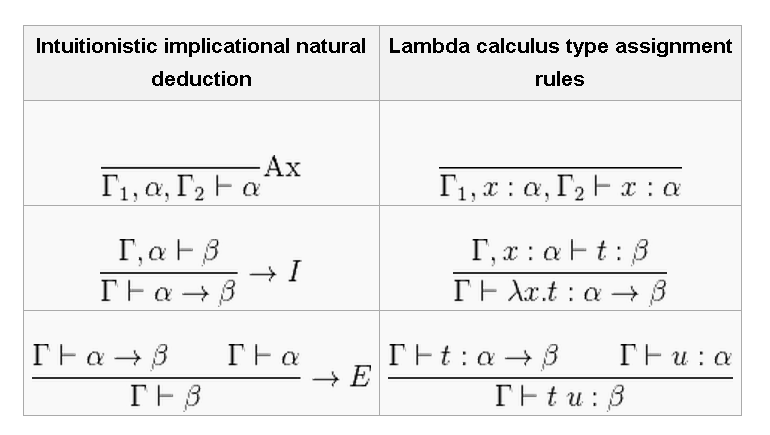
\includegraphics[width=11cm]{curryhoward.png}
\end{frame}


\SlideSection{Conclusions}
\SlideSubSection{Conclusions}
\begin{slide}{
\item Where does this leave us?
\pause
\item Crying in a corner:
\begin{itemize}
\item mathematics and informatics are isomorphic
\item mathematics and informatics are structurally unable of providing absolutely perfect answers to some questions
\item the choice of formalism, language, etc. does not change this
\item different formalisms matter for humans, but not for the underlying knowledge
\end{itemize}
}\end{slide}

\begin{slide}{
\item We cannot solve the problem
\item But we can approximate the heck out of it
\item \textit{Abstract interpretation}, \textit{dependent types}, etc.
\item Hopefully the \textit{interesting, regular} programs are the only ones that we care about
}\end{slide}

\begin{frame}{Dit is het}
\center
\fontsize{18pt}{7.2}\selectfont
The best of luck, and thanks for the attention!
\end{frame}

\end{document}
